% file: main.tex
\documentclass[10pt,oneside]{journal}
\usepackage{mathtools}
\usepackage{fullpage}
\usepackage{listings}
\usepackage{color}
\usepackage{float}
\usepackage{graphicx}
\usepackage[space]{grffile}
 
\definecolor{dkgreen}{rgb}{0,0.6,0}
\definecolor{gray}{rgb}{0.5,0.5,0.5}
\definecolor{mauve}{rgb}{0.58,0,0.82}
\definecolor{dkred}{rgb}{0.7,0,0}




\lstset{ %
  language=Python,                % the language of the code
  basicstyle=\small,              % the size of the fonts that are used for the code
  numbers=left,                   % where to put the line-numbers
  numberstyle=\small\color{gray},  % the style that is used for the line-numbers
  stepnumber=1,                   % the step between two line-numbers. If it's 1, each line 
                                  % will be numbered
  numbersep=5pt,                  % how far the line-numbers are from the code
  backgroundcolor=\color{white},      % choose the background color. You must add \usepackage{color}
  showspaces=false,               % show spaces adding particular underscores
  showstringspaces=false,         % underline spaces within strings
  showtabs=false,                 % show tabs within strings adding particular underscores
  frame=single,                   % adds a frame around the code
  rulecolor=\color{black},        % if not set, the frame-color may be changed on line-breaks within not-black text (e.g. commens (green here))
  tabsize=4,                      % sets default tabsize to 2 spaces
  captionpos=b,                   % sets the caption-position to bottom
  breaklines=true,                % sets automatic line breaking
  breakatwhitespace=false,        % sets if automatic breaks should only happen at whitespace
  title=\lstname,                   % show the filename of files included with \lstinputlisting;
                                  % also try caption instead of title
  keywordstyle=\color{blue},          % keyword style
  commentstyle=\color{dkgreen},       % comment style
  stringstyle=\color{mauve},         % string literal style
  escapeinside={\%*}{*)},            % if you want to add a comment within your code
  morekeywords={class,private,procedure,device},               % if you want to add more keywords to the set
  emphstyle=\color{dkred},
  emph={MPI_BCAST,MPI_INTEGER,MPI_COMM_WORLD,ierror,MPI_RECV,MPI_SEND,MPI_DOUBLE_PRECISION,MPI_SCATTER,MPI_GATHER,MPI_INIT,MPI_COMM_SIZE,MPI_COMM_RANK,MPI_WTIME,MPI_BARRIER}
}

\begin{document}
	
	%!TEX root = ../main.tex
% file: title.tex
\begin{center}
\textsc{\Large MCS507 Project Two:\\}
\textsc{Study a Mathematical Software Package: Earth}
\end{center}
\begin{minipage}{0.6\textwidth}
\begin{flushleft}
	Prepared By: Adam McElhinney
\end{flushleft}
\end{minipage}
\begin{minipage}{0.39\textwidth}
\begin{flushright}
	October 28, 2012
\end{flushright}
\end{minipage}\\[0.01in]
\hrule
	
    %!TEX root = ../main.tex
% file: assignment2.tex


\graphicspath{{C:/Documents and Settings/amcelhinney/My Documents/GitHub/MCS507ProjectTwo/tex/include/}}

\section{Assignment One: Overview and Illustrative Example.} % (fold)
\label{sec: Main Problem}
Our first objective is to identify the main problem this software aims to solve. We then provide an overview of the software package and the algorithms used. We conclude with an illustrative example that displays the utility of this software.

\subsection{Main Problem this Software Aims to Solve} % (fold)
\label{sub:methoda}
The Earth software package is an implementation of the Multivariate Adaptive Regression Splines (MARS) technique developed by Jerome H. Friedman of Stanford University. Interestingly, the reference MARS is copywritten, thus open source implementations of the software are referred to as Earth. The purpose of this technique is similar to that of all regression techniques, namely to fit a function to a set of data. However, the Earth software specifically seeks to do this in a manner that has the following advantages:
\begin{enumerate}
\item Ability to easily handle non-linear data sets
\item Ease of interpretation 
\item Ability to handle large datasets
\item Automatic variable selection
\end{enumerate}


% subsection Main Problem this Software Aims to Solve (end)

\subsection{Overview of the Software and Algorithms} % (fold)
The Earth software package relies on the application of splines to construct the function to predict the target variable. Broadly speaking, a “spline” is simply a function constructed in various segments from other polynomial functions. The MARS technique relies on a type of splines known as hinge functions, which can be represented in the form:  

\begin{equation}
h_{j}=\max (0,x-c)
\end{equation}

The constant c is referred to as the knot. The Earth software then uses these functions to divide the data into mutually exclusive segments and then fit a model to each individual function. This is done in such a manner as to minimize some objective function. One commonly used objective function is the residual sum of squares (RSS).

\begin{equation}
RSS=\sum_{i=1}^{n} (y_{i}-f(x_{i}))^{2}
\end{equation}

To illustrate, let us consider the typical regression equation where we seek to build a model that predicts the value of the $y_{i}$-th obvseration based on some values of $x$.

\begin{equation}
y_{i}=\beta _{0}+\sum_{i=1}^{M}\beta _{i}*x_{i}
\end{equation}

The Earth software then modifies this model to have the following form (where $h_{i}$ represents the hinge function in equation 1).

\begin{equation}
y_{i}=\beta _{0}+\sum_{i=1}^{M}\beta _{i}*h_{i}(x_{i})
\end{equation}

To fit this model, the Earth software relies on two distinct steps.
\begin{enumerate}


\item Forward Pass: In this step, the model starts with just one intercept term composed of the mean of the target (y) variables. Then the software divides the data into two distinct sets via a pair of basis functions. The area dividing point between these two areas is the knot referred to in equation 1. The position of this knot is calcuated such that it results in the maximum reduction in the $RSS$ in equation 2. This process is repeated until the software has reached a maximum number of terms (as defined by the user prior to initializing the model), or until the change in $RSS$ is too small to continue.

\item Backward Pass: The result of the first step will be a model that fits the data set extremely closely, however it is likely that the model will generalize well to other data. Thus, the backward pass (sometimes referred to as pruning) is applied. In this step, the model searches for the basis functions that contribute to the smallest increase in the goodness of fit. However, the $RSS$ will always favor a model with more parameters, so a goodness of fit measure that penalizes additional parameters is needed. This is referred to as the Generalized Cross Validation $GCV$.



\begin{equation}
GCV=\frac{\sum_{i=1}^{n} (y_{i}-f(x_{i}))^{2}}{1-\frac{C}{n}}
\end{equation}

where $C=1+c*d$, $n$ is the number of observations in the data, $d$ is the number of independent basis functions and $c$ is a penality for adding a basis function.
 
\end{enumerate}


% subsection Overview of the Software and Algorithms (end)


\subsection{Illustrative Example of the Earth Software} % (fold)

To illustrate usage of the Earth software, a simple example data set was generated using the Data Painter tool from the Orange Machine Learning Python library. This data set is composed of an $x$ variable which we attempt to use to predict the value of the $y$ variable. We begin by loading the data, verifying the column names, and then inspect the data.

\begin{lstlisting}[caption={Load and Inspect the Data},label=lst:expected_times,firstnumber=15]

  # Remember to add the "class" keyword to the third line, under the target variable. See here:
  # http://orange.biolab.si/doc/tutorial/load-data/
  data = orange.ExampleTable("painted_data_wo_outlier")
  print data.domain.attributes
  print data[:4]
\end{lstlisting}

After reviewing the data, we convert it to \emph{Numpy} arrays and plot the data using \emph{Matplotlib}.

\begin{lstlisting}[caption={Convert to Array and Plot},label=2nd,firstnumber=21]
X, Y = data.to_numpy("A/C")

pl.plot(X, Y, ".r")
pl.title('Example Data Set')
pl.show()

\end{lstlisting}



\begin{figure}[H]
    \centering
       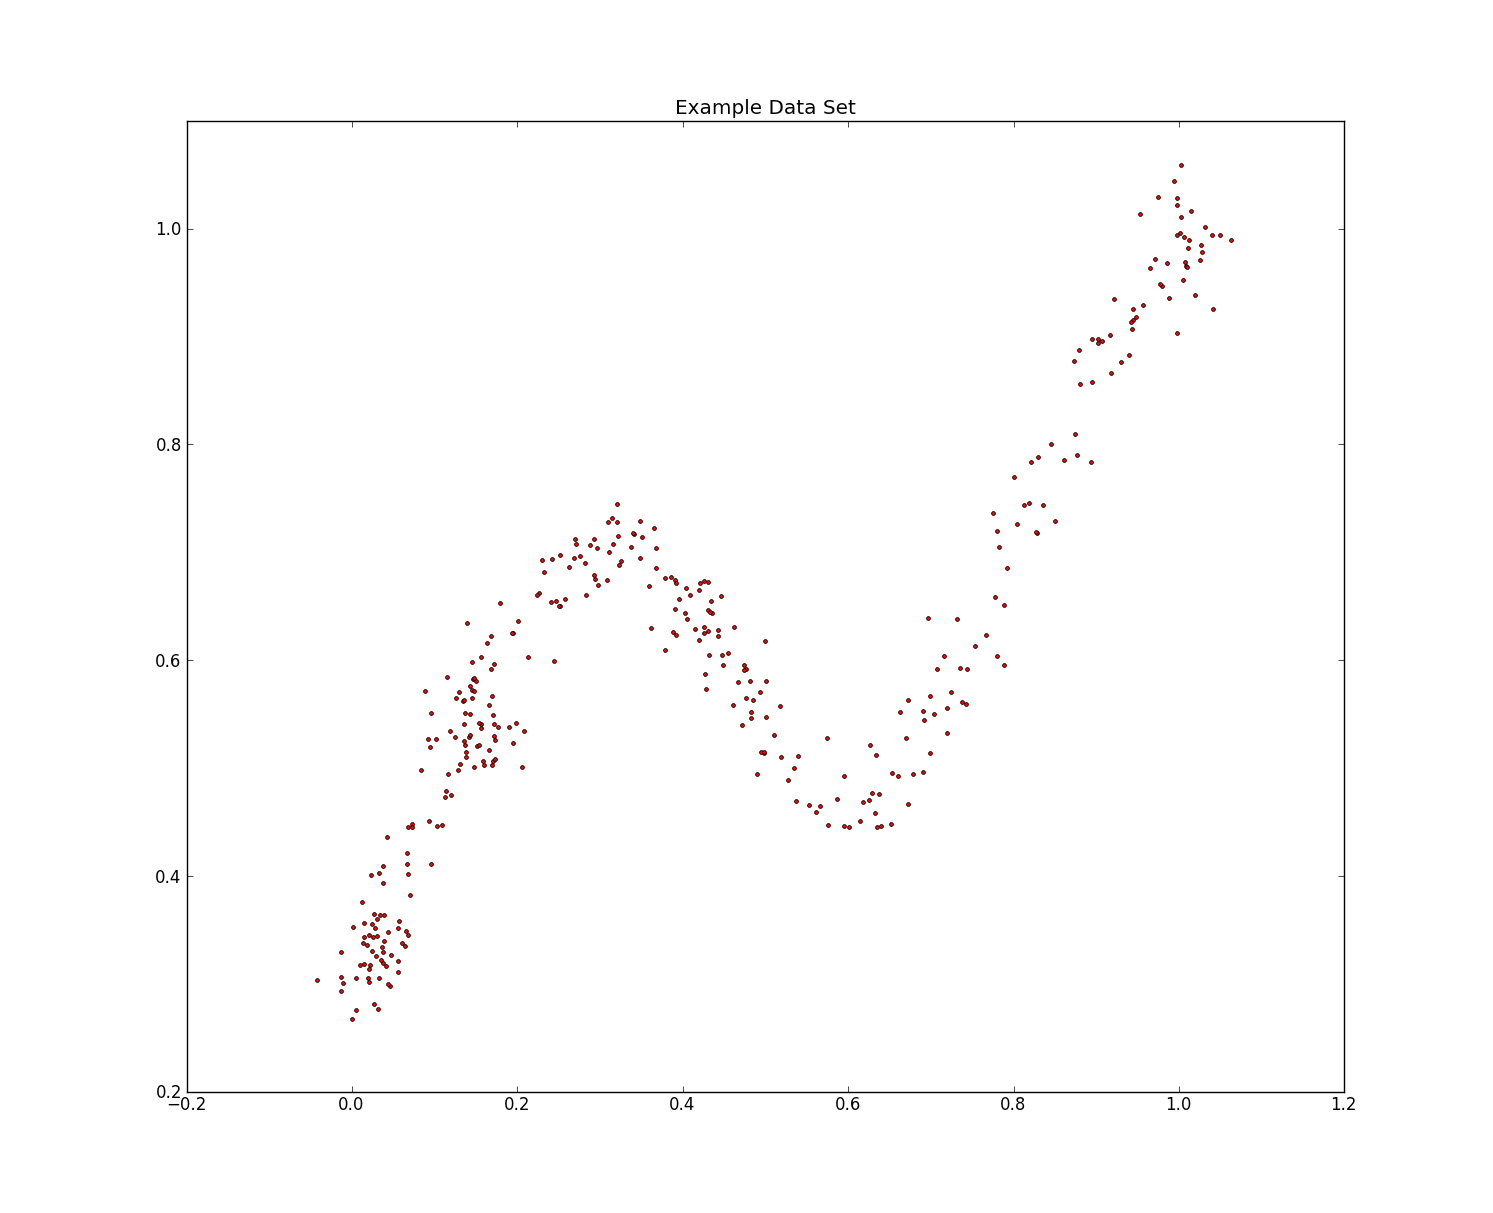
\includegraphics[width=6.5in]{example_data.png}
    \caption{Example Data}
    \label{Example Data}
\end{figure}

As can be seen from the graph, the data exhibits an irregular shape and the density of the points varies as one moves along the x-axis. Thus, this example should prove interesting to test to utility of the Earth software. Next, we use Earth to fit the data and examine the model. 

\begin{lstlisting}[caption={Fit the Data},label=3rd,firstnumber=27]
earth_predictor = earth.EarthLearner(data)
print earth_predictor

\end{lstlisting}

\begin{equation}
	Y =   1.486   +1.445 * \max (0, X - 0.744)   -1.590 * \max (0, 0.744 - X)   -1.818 * \max (0, X - 0.244)
\end{equation}
\begin{equation}
\nonumber
	+2.625 * \max (0, X - 0.640)   -0.682 * \max (0, X - 0.404)   -1.661 * \max (0, X - 0.979)
\end{equation}


Next, we would like to see how well this model predicts the data. One strategy is to plot the values the Earth model predicts and compare them with the actual data. This is done by creating a \emph{Numpy} array of $x$-values and then using the Earth model to predict the values of $y$.

\begin{lstlisting}[caption={Compare the Predicted vs Actual Values and Plot the Results},label=2nd,firstnumber=29]
earth_predictor = earth.EarthLearner(data)
print earth_predictor
linspace = numpy.linspace(min(X), max(X), 20)
predictions = [earth_predictor([s, "?"]) for s in linspace]
pl.plot(X, Y, ".r")
pl.plot(linspace, predictions, "-b")
pl.title('Example Data Set with Line Fit by MARS')
pl.show()
\end{lstlisting}

\begin{figure}[H]
    \centering
       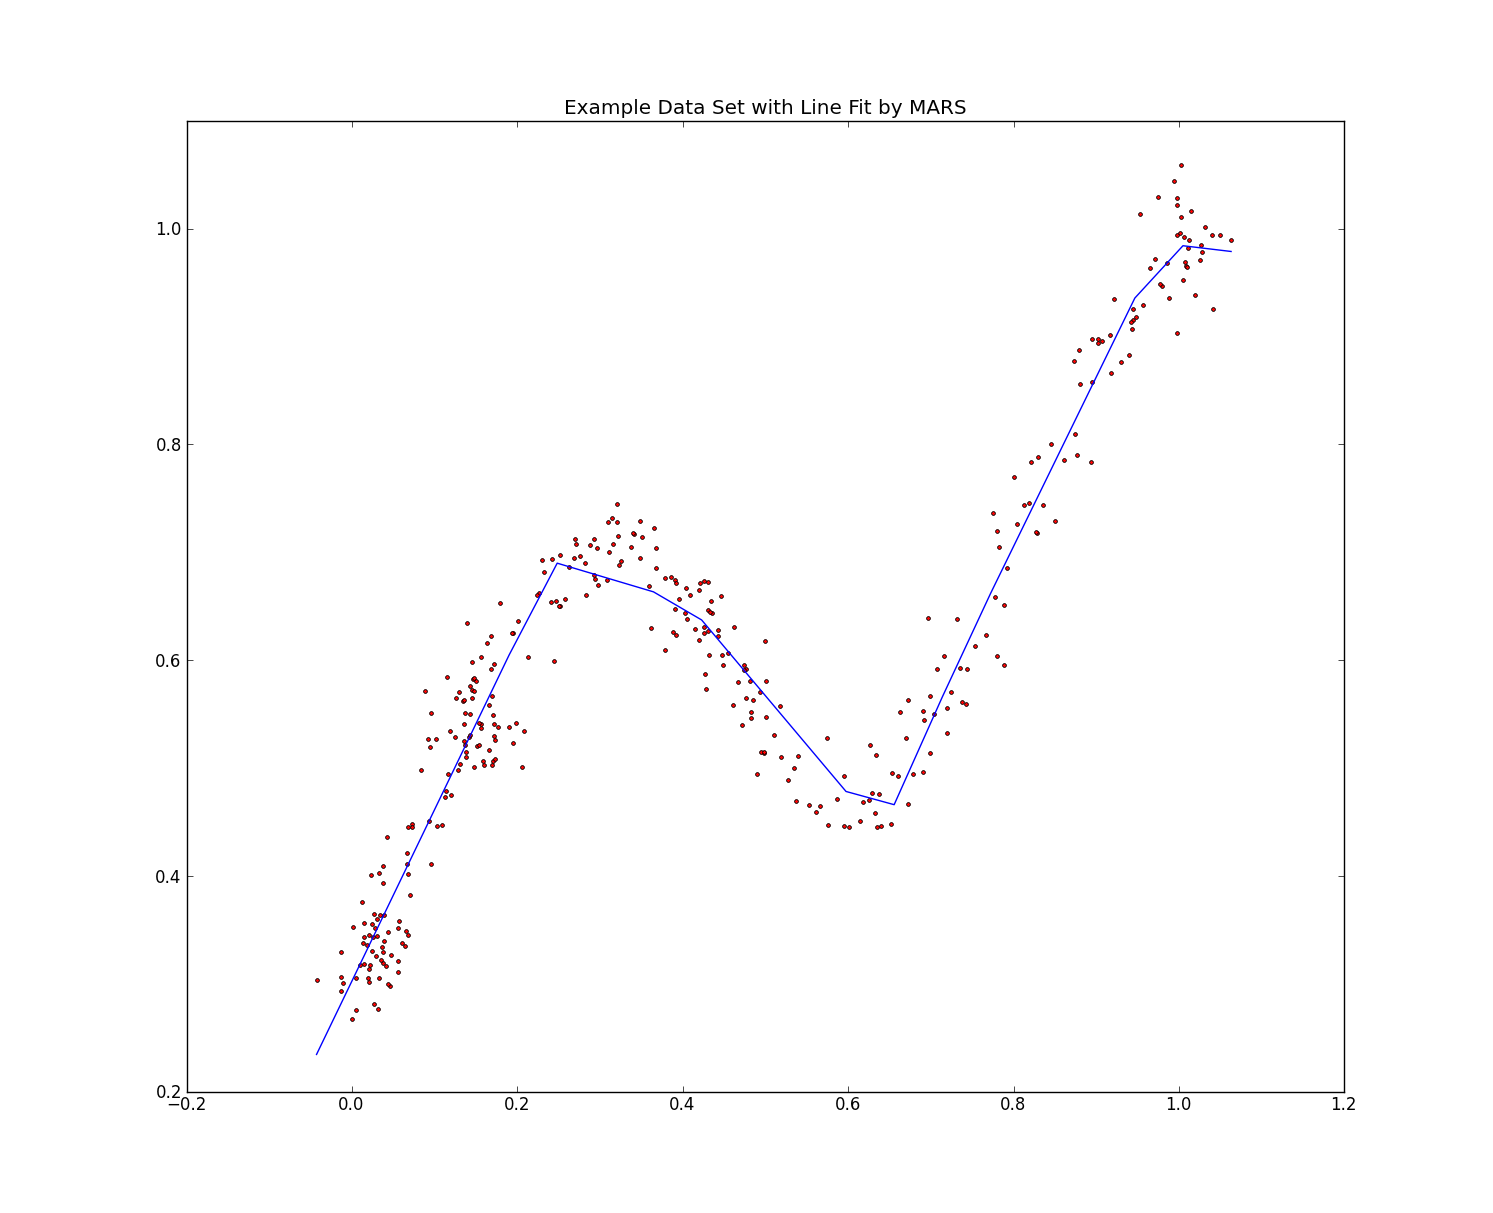
\includegraphics[width=6.5in]{example_data_fit.png}
    \caption{Example Data Set with Line Fit by MARS}
    \label{Example Data}
\end{figure}

Figure 2 shows us that the model output by the Earth software fits the data quite well. It appears that the knots are located close to the inflection points in the data.






% section section_name (end)

    %!TEX root = ../main.tex
% file: assignment2.tex


\graphicspath{{C:/Documents and Settings/amcelhinney/My Documents/GitHub/MCS507ProjectTwo/tex/include/}}

\section{Assignment Two: Using the Software from Python and Extending Illustrative Example} % (fold)
\label{sec: First}
Our second objective is to review how to utilize this software from Python. We then extend the illustrative example from Assignment One to further display the advantages and disadvantages of the Earth software.

\subsection{Utilizing the Earth Software from Python} % (fold)
\label{sub:methoda}
The Earth software is created by Stephen Milborrow and runs in an R environment. R is an open source enviroment for statistical computer. Interestingly, the R language is an extension of a language developed at Bell Laboratories in the late 1970's and early 1980's. Although the Earth software runs in R, it is also available as a standalone program and as a C library. 

Access to the Earth software from Python is done via the Orange module, which is a module focused on data mining and machine learning. It is also available as a standalone software program complete with a GUI. The Orange module and software is developed by the Bioinformatics Laboratory at the Faculty of Computer and Information Science in the University of Ljubljana, Slovenia (Orange Documentation, 10/20/2012). In addition to the implementation of the Earth software, the Orange module features implementations of the majority of cutting-edge machine learning and data mining techniques, including techniques from the following categories:

\begin{enumerate}
\item Summary Statistics
\item Classification
\item Regression
\item Ensemble Algorithms
\item Clustering
\item Network Analysis
\end{enumerate}

\subsection{Extending the Illustrative Example} 

We now seek to extend our Illustrative Example from Assignment One. The natural question arries, "How does the Earth software compare with other traditional techniques?" To answer this question, we utilize the \emph{polyfit} functions from the \emph{NumPy} module to fit polynomial functions of the 3rd, 4th and 5th degrees. We then plot the predicted versus actual values and compare them to the Earth software.

\begin{lstlisting}[caption={Fit Polynomial Functions of the 3rd, 4th and 5th Degrees.  },label=lst:expected_times,firstnumber=43]
p3=polyfit(x,y,3)
pp3=poly1d(p3)

p4=polyfit(x,y,4)
pp4=poly1d(p4)

p5=polyfit(x,y,5)
pp5=poly1d(p5)

pl.plot(X, Y, ".r")
pl.plot(linspace, predictions, "-b")
pl.plot(linspace,pp3(linspace),"-g")
pl.plot(linspace,pp4(linspace),"-m")
pl.plot(linspace,pp5(linspace),"-y")
pl.title('Example Data Set with Line Fit by MARS and Higher Order Polynomials')
pl.legend(['Data','Mars','3rd Degree','4th Degree','5th Degree'],loc=2)
pl.show()
\end{lstlisting}
\begin{figure}[H]
    \centering
       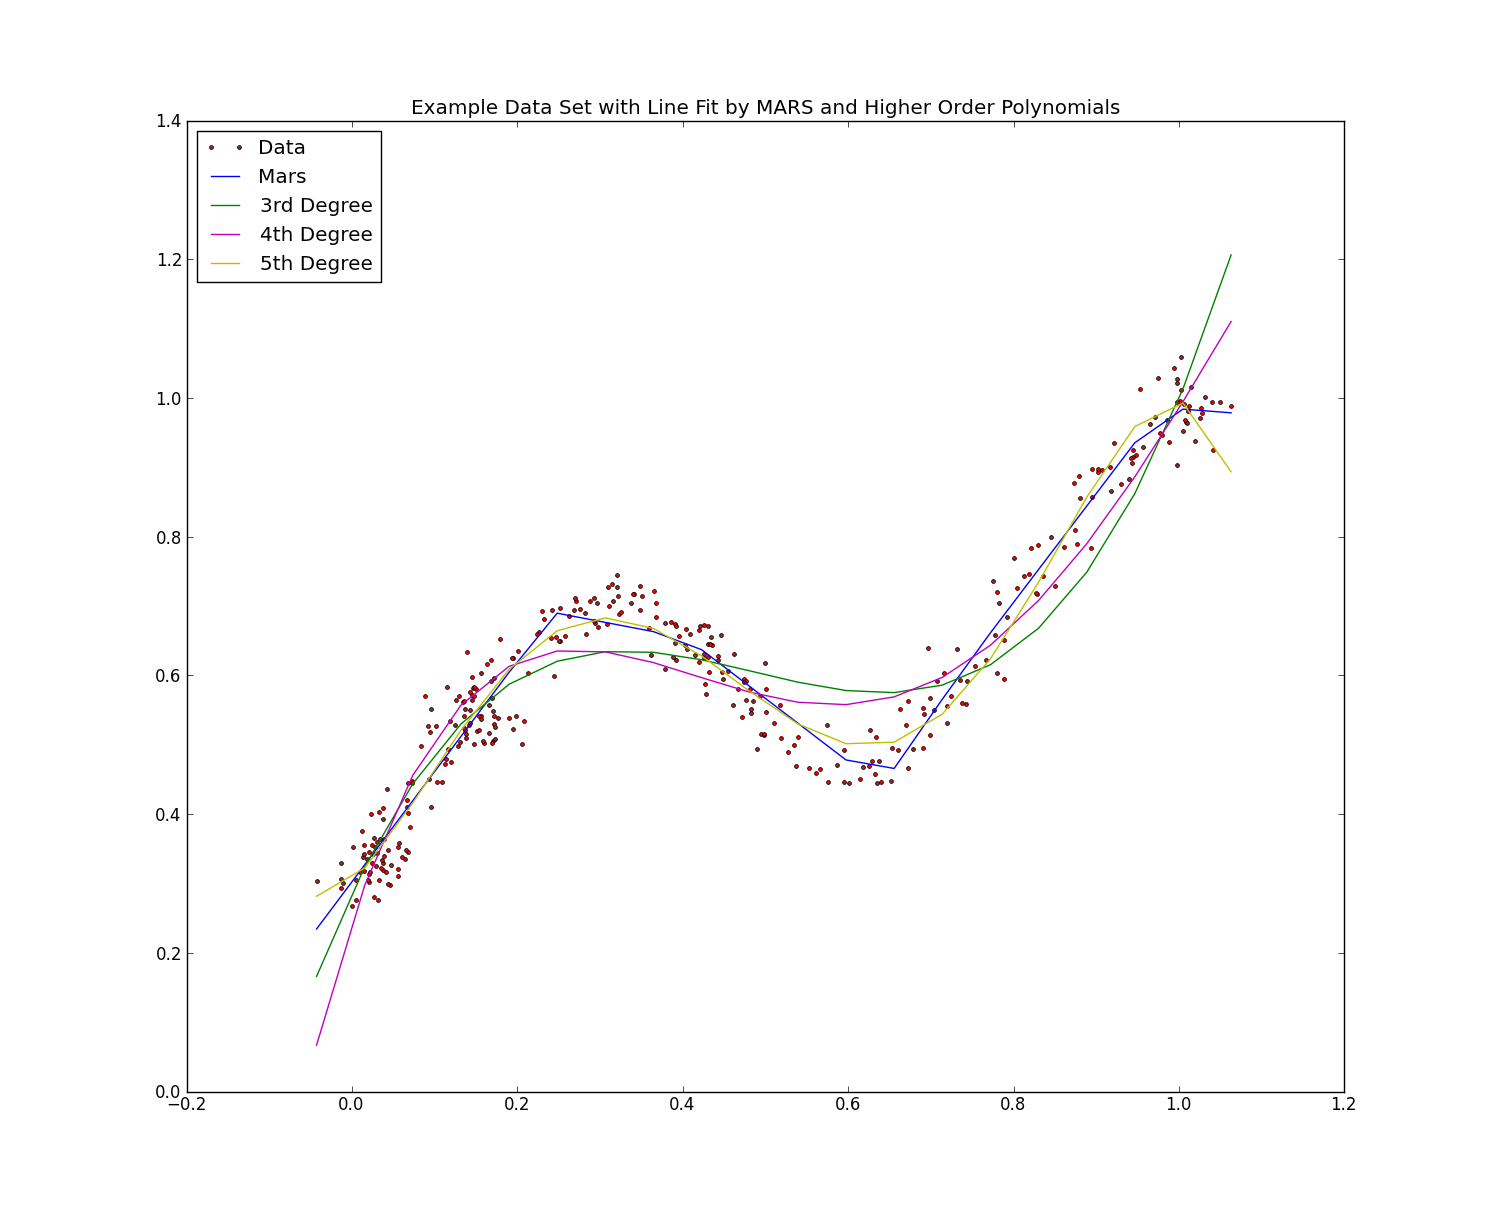
\includegraphics[width=6.5in]{example_data_poly_fit.png}
    \caption{Comparison of the Fit of Mars vs Polynomial Functions}
    \label{Example Data}
\end{figure}

As Figure 3 shows, visually it appears that the Mars model fitted via the Earth software has closer fit than the polynomial functions. Further, the reader should bear in mind that the fitting of the polynomial functions would not be automatic and requires manual input from the modeler, versus the Earth software which automatically selects the best model structure. To empirically test the fit of the 4 models, we define a function to compute the $RSS$. 

\begin{lstlisting}[caption={Calculate the $RSS$ for the Four Models  },label=lst:expected_times,firstnumber=63]
# Create function to calc RSS
def rss(y_obs, y_predicted):
    r=0
    for i in range(len(y_obs)):
        t=(y_obs[i]-y_predicted[i])**2.
        r=r+t
    return r

# Calc RSS for all models
y_predicted1=[earth_predictor([X[i], "?"]) for i in range(len(X))]
y_predicted3=pp3(X)
y_predicted4=pp4(X)
y_predicted5=pp5(X)

r1=rss(Y,y_predicted1)
r3=rss(Y,y_predicted3)
r4=rss(Y,y_predicted4)
r5=rss(Y,y_predicted5)
\end{lstlisting}

\begin{table}[H]
\caption{$RSS$ For the Four Models}
\centering
\begin{tabular}{c c}
\hline\hline
Method & $RSS$ \\
\hline
MARS & 0.59 \\
3rd Degree & 1.57 \\
4th Degree & 1.32 \\
5th Degree & 0.60 \\
\hline
\end{tabular}
\label{table:nonlin} 
\end{table}

As Table 1 shows, the MARS model has the lowest $RSS$, indicating superior fit as compared to the 3 other competing models.

    %!TEX root = ../main.tex
% file: assignment2.tex


\graphicspath{{C:/Documents and Settings/amcelhinney/My Documents/GitHub/MCS507ProjectTwo/tex/include/}}

\section{Assignment Three: More Challenging Inputs and Examples} % (fold)
\label{sec: First}


\subsection{The Boston Housing Data Set} % (fold)
\label{sub:methoda}
To provide a more interesting data set to examine the Earth software implementation of the MARS algorithm, we sought assistance from the UCI Machine Learning Repository which publishes numerous data sets for the benefit of researchers. We chose the Boston Housing Data Set, which is a famous data set outlining housing prices in suburban Boston. The data set contains the following variables:

\begin{enumerate}
\item CRIM: per capita crime rate by town
\item ZN: proportion of residential land zoned for lots over 25,000 sq.ft.
\item INDUS: proportion of non-retail business acres per town
\item CHAS: Charles River dummy variable (= 1 if tract bounds river; 0 otherwise)
\item NOX: nitric oxides concentration (parts per 10 million)
\item RM: average number of rooms per dwelling
\item AGE: proportion of owner-occupied units built prior to 1940
\item DIS: weighted distances to five Boston employment centres
\item RAD: index of accessibility to radial highways
\item TAX: full-value property-tax rate per \$10,000
\item PTRATIO: pupil-teacher ratio by town
\item B: $1000(Bk - 0.63)^{2}$ where Bk is the proportion of blacks by town
\item LSTAT: \% lower status of the population
\item MEDV: Median value of owner-occupied homes in \$1000's
\end{enumerate}

This data set was chosen for the following reasons:
\begin{enumerate}
\item The dataset contains categorical, integer and real variables
\item The number of instances ($n=506$) and the number of attributes ($m=14$) is representative of many typical real-world data sets
\item The data set does not contain missing values, which the MARS algorithm does not address in its basic form
\end{enumerate}

To begin the analysis, we first load in the data. Then, to explore the data set, we constructed a function to compute scatter plots of all the data versus the target variable. 
\begin{lstlisting}[caption={Load the Data and Explore},label=2nd,firstnumber=25]
# Bring in the data using the C4.5 format, which brings in the .data file and then the .names file
data = orange.ExampleTable("housing")
print data.domain.attributes

names=str(data.domain).replace('[','').replace(']','').split(',')
# Make Scatterplots of all the variables versus the target variable
def scatterplot(data, data_name, target_var):
    import matplotlib.pyplot as plt
    M = len(data[0])-1
    N=len(data)
    fig = plt.figure()

    y=[float(data[l][target_var]) for l in range(N)]

    for i in range(M):
        ax = fig.add_subplot(int(M/4.)+1,4,i+1)
        py.setp(ax.get_xticklabels(), visible=False)
        x=[float(data[k][i]) for k in range(N)]
        ax.scatter(x,y)
        #ax.set_xlabel(data_name[i],size='10')
        ax.set_title(data_name[i],size='10')
        #ax.set_ylabel(data_name[target_var],size='10')
    return fig
fig = scatterplot(data, names, len(data[0])-1)
\end{lstlisting}

\begin{figure}[H]
    \centering
       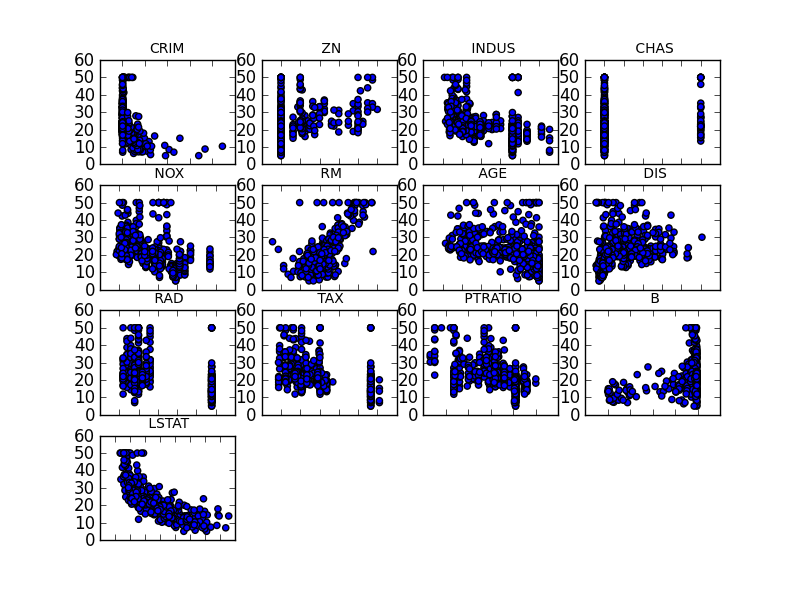
\includegraphics[width=6.5in]{scatter.png}
    \caption{Scatterplot of the Independent Variables vs the Target Variable}
    \label{Example Data}
\end{figure}

\subsection{Fitting the MARS Model} % (fold)

Simiarly to previous examples, the Earth software lets us very quickly view the data, fit the data to the model and then view the model. 
\begin{lstlisting}[caption={Load the Data and Explore},label=2nd,firstnumber=53]
# View the data
for i in range(5):
    print data[i]


earth_predictor = earth.EarthLearner(data)

print earth_predictor
\end{lstlisting}

\begin{equation}
	MEDV =
   33.518
   -0.687 * \max(0, CRIM - 4.422)
   -1.132 * \max(0, 4.422 - CRIM)
\end{equation}
\begin{equation}
\nonumber
+0.560 * \max(0, CRIM - 12.048)-28.029 * \max(0, NOX - 0.488)+7.127 * \max(0, RM - 6.431)
\end{equation}
\begin{equation}
\nonumber
   -0.662 * \max(0, DIS - 2.436)
   +5.010 * \max(0, 2.436 - DIS)
   +0.031 * \max(0, 296.000 - TAX)
\end{equation}
\begin{equation}
\nonumber
-0.637 * \max(0, PTRATIO - 14.700)
   +1.692 * \max(0, 14.700 - PTRATIO)
   -0.355 * \max(0, B - 393.360)
\end{equation}
\begin{equation}
\nonumber
-0.007 * \max(0, 393.360 - B)
   -0.598 * \max(0, LSTAT - 6.120)
\end{equation}
\begin{equation}
\nonumber
   +2.428 * \max(0, 6.120 - LSTAT)
   +0.716 * \max(0, LSTAT - 25.790)
\end{equation}

We then score the data and utilize our previous function to compute the $RSS$ 
\begin{lstlisting}[caption={Compute the RSS},label=2nd,firstnumber=62]
dl=list(data)

# Predict all the data
y_hat=[]
for i in range(0,len(dl)):
    t=earth_predictor.predict(dl[i])
    y_hat.append(t[0])

os.chdir("C:/Documents and Settings/amcelhinney/My Documents/GitHub/MCS507ProjectTwo/src/")
from earth_example import rss
X, Y = data.to_numpy("A/C")

y_1=rss(Y,y_hat)
\end{lstlisting}
The Earth software also allows us to compute and graph the relative importance of each of the variables on the target variable via the \emph{evimp} and \emph{plot\_evimp} methods.
\begin{lstlisting}[caption={Load the Data and Explore},label=2nd,firstnumber=75]
Orange.regression.earth.plot_evimp(earth_predictor.evimp())
\end{lstlisting}
As the graph below shows, the number of rooms the house has (variable $RM$) and the percentage of the population that is lower status in a given area (variable $LSTAT$) are by far the two strongest predictors of housing price. 
\begin{figure}[H]
    \centering
       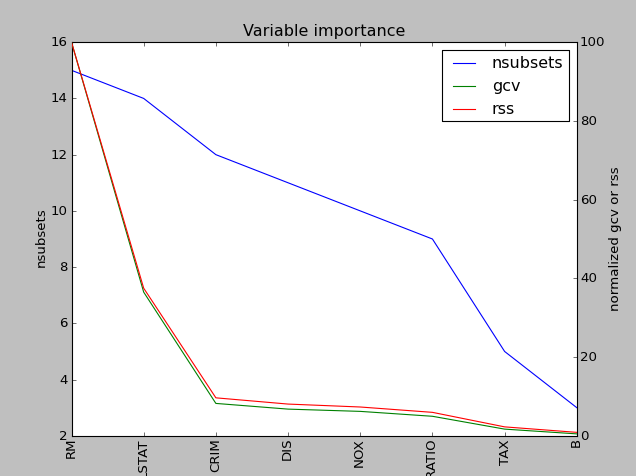
\includegraphics[width=4.in]{variable_importance.png}
    \caption{Relative Importance of the Independent Variables on the Target Variable}
    \label{Example Data}
\end{figure}

Similarly to Assignment 2, we compare the performance of the MARS algorithm versus the traditional least squares regression. However, this time we utilize the \emph{OLS} class from the \emph{SciPy} module. 
\begin{lstlisting}[caption={Fit the OLS Model},label=2nd,firstnumber=77]
# Compute using the standard regression model
import ols
model=ols.ols(Y,X,names[len(names)-1],names[:len(names)-1])
model.summary()
\end{lstlisting}

Unlike the regression fitting packages used in Example 2, the \emph{Ols} class provides us with a full regression output, similar to what one would find in R, SAS, or any other dedicated statistics package.
\begin{figure}[H]
    \centering
       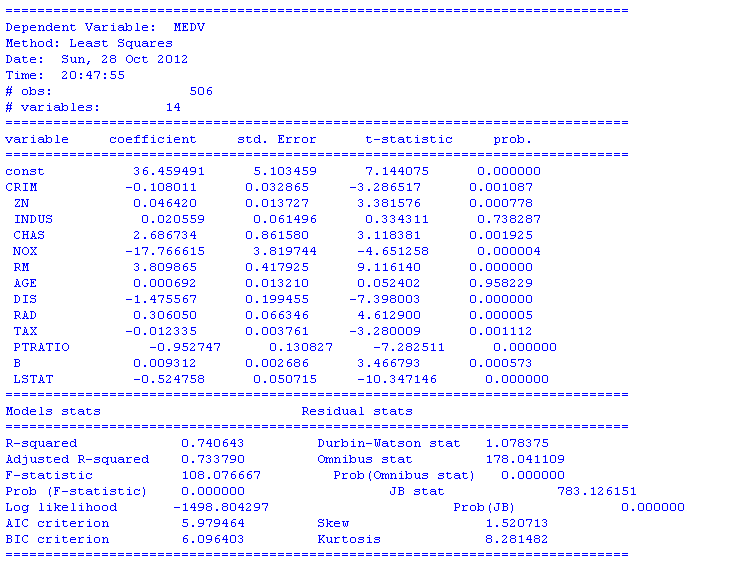
\includegraphics[width=6.5in]{ols_output.png}
    \caption{Output from the \emph{Ols} Class in \emph{SciPy}}
    \label{Example Data}
\end{figure}

Interestingly, the t-statistics for the $RM$ and $LSTAT$ variables are among the largest. This is in alignment with the graph of relative variable importance examined previously. 
\begin{lstlisting}[caption={Calculate the RSS for the OLS Model},label=2nd,firstnumber=83]
# Get the regression coefficients
coeff=model.b
# Score the data
y_hat_ols=[]
for i in range(len(data)):
    y_hat=coeff[0]
    for j in range(len(coeff)-1):
        #print coeff[j+1]
        #print data[i][j]
        y_hat=y_hat+data[i][j]*coeff[j+1]
    y_hat_ols.append(y_hat)
# Compute the RSS
y_2=rss(Y,y_hat_ols)

\end{lstlisting}
Again following the convention from Example 2, we score the data using the OLS Model and compute the $RSS$. 
\begin{table}[H]
\caption{$RSS$ For MARS vs OLS}
\centering
\begin{tabular}{c c}
\hline\hline
Method & $RSS$ \\
\hline
MARS &6311 \\
OLS & 11079 \\
\hline
\end{tabular}
\label{table:nonlin} 
\end{table}
Once again the Earth software shows its utility because the MARS algorithm was better able to predict the target variable as compared to the OLS.

    %!TEX root = ../main.tex
% file: assignment2.tex


\graphicspath{{C:/Documents and Settings/amcelhinney/My Documents/GitHub/MCS507ProjectTwo/tex/include/}}

\section{Conclusion} % (fold)
We have shown how the Earth software package implements the MARS algorithm and how it can be very useful for quickly solving real world problems. We demonstrated how it easily beats least squares regression, while requiring less work from the actual modeler. However, this is by no means a definitive answer. Some factors beyond the scope of this assignment, but relevant for future inquiry are:
\begin{enumerate}
\item Execution time (particularly on large data sets)
\item High dimensional data (data sets where there are a much larger amount of explanatory variables as compared with the number of observations)
\item Various variable transformations and their ability to improve the quality of the OLS models
\item Calculating statistical significance and variance with the MARS model
\item Available heuristics to improve MARS calculation time, including the Fast Mars model
\item Utilizing MARS for purposes of classification 
\item Implementing our own MARS algorithm and comparing performance to that of the Earth software
\end{enumerate}

In summation, the Earth software package is a cross-platform, versatile tool with applications to real world data sets. It should be considered by any modeler seeking a fast, intuitive and accurate regression modeling technique.
    \input{include/bibliograph.tex}
	

	
	
\end{document}